\section{Visió global}
\label{arquitectura:visio_global}
%\textbf{Oscar}:\textit{Visió general del diseny (que fa el front end i que fa el backend, en general) (tipic grafic de 3 capes front/back/dades) Aqui haurás de posar diseny de la BD, suposo que el cas d'us general (posa els ninotets de enginyeria del software i com interactuen amb el sistema, el flux d'execució) i en el backend fes capsetes amb els moduls}
Si prenem el projecte d'aquest TFG des d'un punt de vista global, sense prendre en consideració els detalls particulars de cada un dels elements que el formen, veiem que respon a l'arquitectura representada a la Figura \ref{fig:arquitectura_global}.
\begin{figure}[h!]
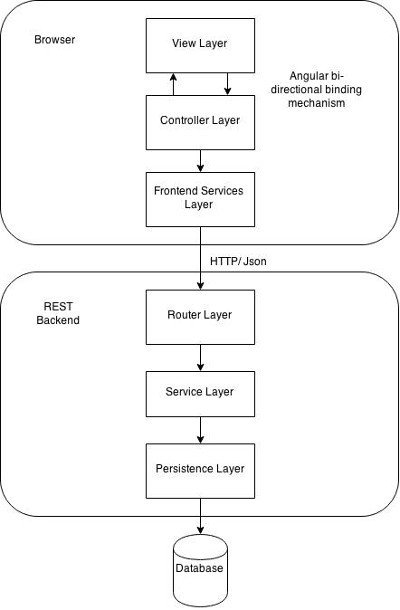
\includegraphics[scale=0.4]{sections/arquitectura/modern_global2.jpg}
\centering
\caption{Arquitectura en tres capes}
\label{fig:arquitectura_global}
\end{figure}
\newline A nivell conceptual, busca independitzar la lògica de negoci, de la lògica de presentació, del model de dades. Podent entendre cada un dels elements com entitats independents, en ocasions amb la seva pròpia arquitectura.\\
\newline En el context del TFG, el projecte està format principalment per dos elements, \textit{frontend} i \textit{backend}, que es comuniquen entre ells mitjançant crides HTTP\footnote{Hypertext Transfer Protocol}.
%En el context concret d'aquest TFG, l'adopció d'aquesta arquitectura es tradueix en un \textit{frontend}, que es comunica mitjançant els mètodes \textit{Get}, \textit{Post}, \textit{Put} i \textit{Delete} del protocol HTTP\footnote{Hypertext Transfer Protocol}, amb un \textit{backend}, que s'encarrega de servir les dades per mostrar.
\subsection{Frontend}
\label{arquitecura:global_frontend}
Correspon a la part client del projecte, a través de la qual l'usuari final interactuarà amb el sistema (visualitzar pdf's, signar documents, etc.).\\
Com s'ha dit anteriorment, es pot interpretar el \textit{frontend} com una entitat independent, i com a entitat independent, disposa de la seva pròpia arquitectura, en aquest cas, arquitectura MVC\footnote{Model View Controller}.
\begin{figure}[h]
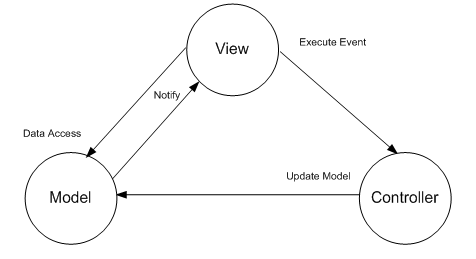
\includegraphics[scale=0.5]{sections/arquitectura/mvc.png}
\centering
\caption{Model-Vista-Controlador}
\label{fig:arquitectura_mvc}
\end{figure}
\newline L'arquitectura, ve donada pel mateix \textit{framework} que s'ha fet servir per al desenvolupament  (AngularJS).\\
\newline Per fer-ne un breu resum, aquesta arquitectura proposa distribuir els elements de codi en tres grups:
\begin{itemize}
    \item \textbf{Model}, representa les dades, s'encarrega de la seva gestió, rebre i servir. En aquest cas concret, s'encarrega de la comunicació amb el \textit{backend}, qui realment té les dades.
    \item \textbf{Vista}, el que veu l'usuari. Captura les interaccions i les transmet cap al controlador per que actui en conseqüència.
    \item \textbf{Controlador}, s'encarrega d'interpretar les interaccions que rep de la vista i modificar la vista en conseqüència.
\end{itemize}
Amb aquesta arquitectura, aconseguim un sistema modularitzat, amb dades sempre actualitzades i capes independents els uns dels altres.
\clearpage
 %donat que el client web no disposa d'\textit{storage} pròpi, entendrem com a model el component dins del projecte que s'encarrega de realitzar les peticions al \textbf{backend} i rebre'n els resultats (ja siguin satisfactoris o no).\\
\subsubsection{Diagrama de casos d'ús}
La tasca del \textit{frontend} és relativament senzilla.\\
Per una banda ha de permetre a l'usuari rebre la informació pertinent en cada cas i en cada moment. Per l'altra, ha de permetre a l'usuari ``jugar'' amb les dades i interactuar-hi.\\
Amb les anteriors premises, la component \textit{frontend} del projecte ha de ser capaç de permetre que l'usuari realitzi un seguit d'accions.\\
\newline La Figura \ref{fig:cas_us_frontend} mostra els casos d'ús (o accions) que necessàriament s'han de poder realitzar:
\begin{figure}[h]
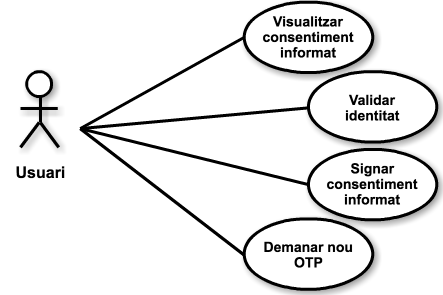
\includegraphics[scale=0.5]{sections/arquitectura/frontend_usecase.png}
\centering
\caption{Casos d'ús \textit{frontend}}
\label{fig:cas_us_frontend}
\end{figure}
\newline L'objectiu principal del \textit{frontend}, és permetre a l'usuari rebre les dades necessàries i donar el \textit{feedback} necessari per saber si l'operació de signatura s'ha dut a terme amb èxit o no.\\
\newline Així doncs, la part client del projecte té els següents propòsits:
\begin{itemize}
    \item Visualitzar consentiment informat:\\
    L'usuari ha de ser capaç de veure el consentiment informat dins de la mateixa plataforma. Alhora, hauria de ser capaç de descarregar-lo.
    \item Validació d'identitat:\\
    Abans de signar el document s'ha de validar la identitat del signant.
    \item Signatura consentiment informat:\\
    El sistema ha de permetre la signatura del document via OTP rebut per SMS.
    \item Demanar nou OTP:\\
    En cas de caducar el el codi enviat en el moment de la validació, l'usuari ha de ser capaç de demanar un nou codi OTP que li permeti signar el consentiment informat.
\end{itemize}
Aquestes quatre operacions, són les que el sistema d'emissió, validació i signatura electrònica de consentiment informats ha de tenir per a satisfer les necessitats bàsiques que es plantegen al projecte.\\
\newline Qualsevol afegit o bé característica addicional, ha de servir per complementar les anteriors.
%\clearpage
%Totes les operacions anteriors, es tradueixen en tot un seguit de crides HTTP a un backend mitjançant els mètodes GET i POST.

%Amb una cerca ràpida a \textit{Google} de la paraula \textit{frontend}, trobem la següent definició sota l'etiqueta \textit{computing}:
%\begin{displayquote}
%"\textit{\textbf{adj.} (of a device or program) directly accessed by the user and allowing access to further devices or programs.}"
%\end{displayquote}
%Tenint en compte l'anterior definició podem sobreentendre que la paraula \textit{frontend} fa referència a la part del projecte amb la que l'usuari interactuarà de forma directe, aquella que ha de permetre el visualitzar, signar i validar els consentiments informats que es generin amb la compra dels serveis a través de la plataforma; i fer-ho de la forma mes usable possible.\\
%\newline El \textit{frontend} s'ha desenvolupat amb \textit{AngularJS}\footnote{https://angularjs.org/}, un dels frameworks Javascript més estesos en el panorama \textit{web-development} actual.

%\subsection{AngularJS}
%\textit{AngularJS} és un framework per al desenvolupament d'aplicacions web dinàmiques, caracteritzat per ser de codi obert, basat en javascript i sobretot, mantingut principalment per \textit{Google} i una àmplia comunitat que s'esforça en donar solució als reptes que sorgeixen en el desenvolupament de les anomenades \textit{SPA} (\textit{Single Page Application}).\\
%\newline Un altre punt que ha posicionat fortament \textit{AngularJS} com un dels \textit{frameworks} per antonomàsia en el que fa a desenvolupament web, és l'us de l'arquitectura MVC (Model Vista Controlador), que ens permet distribuïr el codi i funcionalitats d'una forma coherent i fàcilment testejable.\\
%\newline Cap a finals de 2016 es va alliberar una versió estable del que s'anomena \textit{Angular2}, una revisió integral del framework web. Aquesta revisió suposa una reescriptura total del mateix, així com el canvi de funcionament de molts mòduls del propi \textit{framework}. Aquest pot ser un dels principals motius que l'adopció d'aquesta segona versió sigui lenta i costosa. \\
%\newline Actualment es consideren versions suportades les versions 2.4.1 i 1.6.1, sent aquesta última la més emprada sempre que es parla d'\textit{AngularJS}.\\
%\newline A grans trets, \textit{AngularJS} extén l'HTML aportant tot un seguit d'etiquetes, anomenades directives, que permeten als desenvolupadors coses com:
%\begin{itemize}
%    \item Control d'estructures del DOM
%    \item Amagar i mostrar elements del DOM
%    \item Validació dinàmica de formularis
%    \item Afegir nous comportaments a elements del DOM (gestió d'events...)
%    \item Reutilitzar HTML  agrupant-lo en components
%\end{itemize}
%\subsubsection{Single Page Application}
%El terme \textit{single page application} (SPA) es fa servir principalment amb aplicacions web que ofereixen un tipus d'interacció dinàmica i semblant al que trobariem en aplicacions mòbils o d'escriptori.\\
%\newline La principal diferècia entre una pàgina web corrent i una \textit{SPA}, és que aquesta última refresca molt poques vegades la pantalla. Una \textit{SPA} fa un ús intensiu d'AJAX, una forma de comunicar-se amb la part back-end servidora sense necessitat de refrescar la pàgina, que permet carregar les dades directament dins de la nostra aplicació, fent que aquestes es renderitzin directament sobre client.\\
%\newline En altres paraules, quan l'usuari accedeix per primera vegada a una \textit{SPA}, el navegador web descarregarà tota l'aplicació. Un cop descarregada, a mesura que l'usuari navegui, l'aplicació anirà descarregant la informació necessària i l'anirà pintant a mesura que faci falta i com faci falta. D'aquesta forma, s'aconsegueix una millor experiència d'usuari, ja que el que l'usuari final 
%\subsubsection{MVC}
%El patró anomenat model vista controlador (mvc) és un patró d'arquitectura del software que proposa el separar els components que formen el software en tres grans blocs. Per una banda el \textbf{model}, que correspon a tots els objectes de la lògica de negoci, també hi ha la \textbf{vista}, altrament dit interfície d'usuari o bé canal de comunicació amb altres programes, i finalment, el \textbf{controlador}, que gestiona tot el flux d'informació així com la comunicació entre el model i la vista.\\
%\newline Portat al context que ens ocupa, \textit{AngularJS}, es tradueix en tot un seguit de vistes, fitxers purament HTML, gestionades per controladors, fitxers Javascript, que vinculen dades i en controlen el comportament, i una bateria de serveis i llibreries, també fitxers Javascript, que són les encarregades de realitzar la comunicació amb el "món exterior".



\clearpage
\subsection{Backend}
\label{arquitecura:global_backend}
Plantejat i desenvolupat com una API Rest que dóna accés als recursos necessàris dins de la base de dades, a través de rutes (o \textit{endpoints}) definides als controladors.\\
\newline L'accés a les dades es fa a través d'HTTP, fent ús dels mètodes \textit{Get}, \textit{Post}, \textit{Put} i \textit{Delete}, amb un funcionament similar al \textit{CRUD}\footnote{\textbf{C}reate \textbf{R}ead, \textbf{U}pdate i \textbf{D}elete} d'una base de dades, però a nivell de recurs.\\
\newline Pel que fa a l'arquitectura pròpiament dita, no se n'aplica una de concreta.\\
Per contra, fa ús de tot un seguit de conceptes d'enginyeria del \textit{software} com \textit{clean architecture} i \textit{SOLID}  que tenen com a objectiu la producció d'un codi net, mantenible i sobre tot, ben estructurat.\\
\subsubsection{Clean Architecture}
\label{arquitectura:back_clean}
\begin{figure}[h]
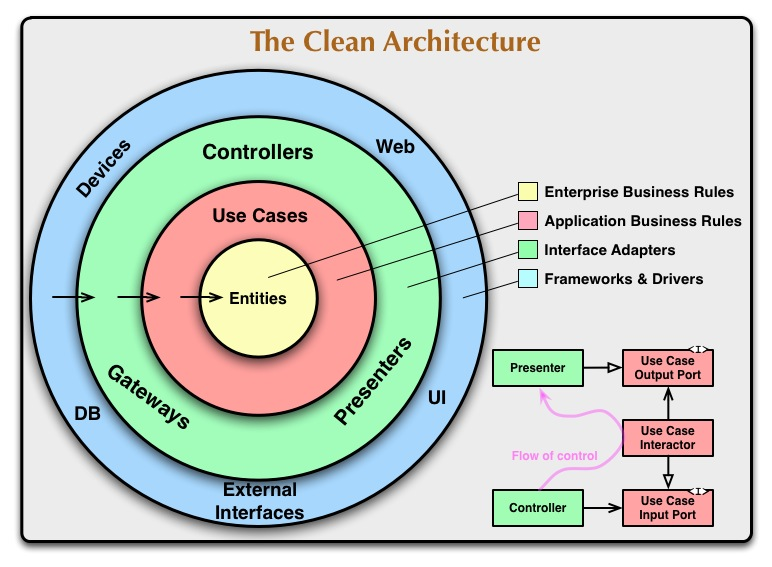
\includegraphics[scale=0.4]{sections/arquitectura/cleanArchitecture.jpg}
\centering
\caption{Clean Architecture}
\label{fig:clean_architecture}
\end{figure}
La figura anterior (Figura \ref{fig:clean_architecture}), ens presenta un model conceptual que rep el nom de \textit{clean architecture}\cite{clean}.% on les diferents capes són independents les unes de les altres, de tal forma que caldrà aplicar tot un seguit d'\textit{adapters} entre capes per poder comunicar-se entre elles.\\
%\newline La capa més interna, no coneix a la capa més externa i viceversa. Aqust fet, provoca una atomicitat tant a nivell conceptual com a nivell de codi bastant notable. \\
%A la llarga, l'atomicitat i el poc solapament aconseguits d'aplicar la filosofía \textit{clean architecture} serà clau per a un bon escalat del projecte.\\
El primer que s'ha de tenir en compte quan es parla d'aquesta arquitectura, és que es regeix pel que s'anomemena \textit{Dependency rule}, segons la qual les capes internes no poden comunicar-se amb les capes externes.\\
\newline Gràcies a aquesta estructura, la lògica de negoci sempre és independent del \textit{framework}, de com s'obtenen o es mostren les dades o altres factors externs.\\
\newline SOLIDi s'ha estructurat el projecte de forma apropiada, no s'ha de patir per si en un futur es canvien tecnologies o llibreries, la lògica de negoci continuarà funcionant exactament igual.
\clearpage
%\newline D'aquesta forma, s'aconsegueix un codi atomitzat, fàcil de mantenir donat el poc solapament que hi ha entre els diferents components del projecte, i amb components fàcilment substituïbles.\\
\subsubsection{S.O.L.I.D}
\label{arquitectura:back_solid}
\cite{solid} És l'acrònim de:
\begin{itemize}
    \item \textit{\textbf{S}ingle responsability}
    \item \textit{\textbf{O}pen close}
    \item \textit{\textbf{L}iskov substitution}
    \item \textit{\textbf{I}nterface segregation}
    \item \textit{\textbf{D}ependency inversion}
\end{itemize}
Els cinc punts anteriors, són un seguit de convencions i idees enfocades a la producció d'un codi net, estructurat i fàcil de mantenir.\\
\newline Per aconseguir-ho, treballa amb idees tal com la responsabilitat única de les classes, classes obertes a l'extensió, però no a la modificació, injecció de dependències, ús de interfícies a mode de contracte, etc.\\
\newline Són tot un seguit de regles que funcionen perfectament amb les idees presentades anteriorment referents a la \textit{Clean Architecture}
\subsubsection{Base de dades}
Tot i que ha patit diversos canvis al llarg del desenvolupament del projecte, el model final de la capa de persistència queda tal que:
\begin{figure}[h]
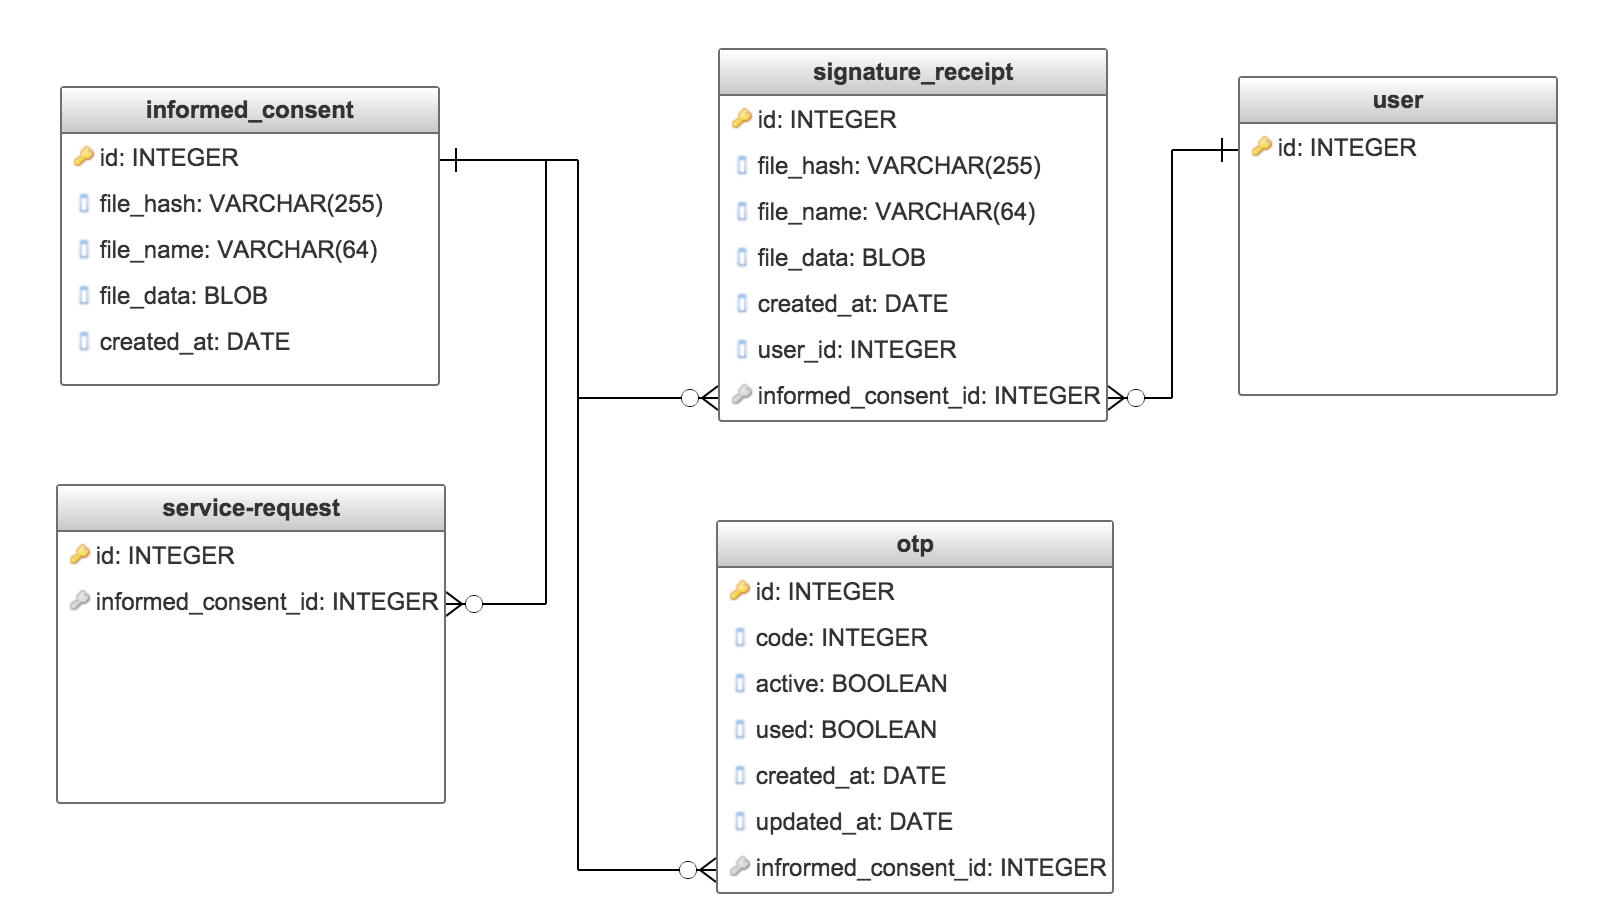
\includegraphics[scale=0.4]{sections/arquitectura/database_model.png}
\centering
\caption{Model de base de dades}
\label{fig:database_model}
\end{figure}
%\begin{itemize}
%    \item Servir les dades al \textit{frontend} sota demanda.
%    \item Realitzar la comunicació amb els serveis externs quan el context això ho demani.
%\end{itemize}

%El \textit{backend} és, en escènica una API Rest que serveix els diferents recursos emmagatzemats a la base de dades (CRUD) per a servir les necessitats que sorgeixin des del \textit{frontend}.\\
%Alhora, realitza la comunicació amb serveis de tercers com \textit{OriginStamp} i \textit{FreeTSA}, necessaris per a garantir el no repudi dels consentiments informats i generats per una segona API privada encarregada de generar tant els consentiments com el comprovant de signatura.\\
%\newline A continuació veurem amb més detall cada un dels components que formen el \textit{backend}:

%\subsection{Nucli}
%Anomenem \textit{nucli} a la API rest a la que el \textit{frontend} llança les diferents crides.
%Aquesta api és un mòdul desenvolupat amb \textit{Symfony}.\\
%\newline \textit{Symfony} és una de les "grans" opcions dins de la extensa llista de \textit{frameworks PHP} existents; alhora que és un dels més emprats per als desenvolupadors per les seves característiques i facilitats, conta amb un renom afegit per ser l'elecció base per a grans projectes com podrien ser el gestor de contingut \textit{Drupal}\footnote{https://www.drupal.org} i \textit{phpBB}\footnote{https://www.phpbb.com/}, un CMS orientat a la creació de fòrums.\\
%\newline Entre les característiques destacades, podem trobar la facilitat d'estructurar el codi, donada la seva clara orientació cap a una arquitectura MVC, així com la re-usabilitat del mateix, sempre i quan es faci ús de bones pràctiques. A tot aixó, \textit{Symfony} conta amb una característica afegida, que també podria ser considerada una facilitat, que és l'ús d'un gestor de dependències per a \textit{PHP} anomenat \textit{Composer}.\\
%De la mateixa manera que hem vist anteriorment al el \textit{frontend}, concretament amb \textit{node.js} i \textit{npm}, \textit{Comsposer} llegeix del fitxer \textit{composer.json} per tal d'instal·lar les dependències del projecte sense necessitat de fer-ho d'una en una, i d'aquesta forma facilitar-ne la migració i el treball col·laboratiu.\\
%\newline Com a característiques de \textit{Symfony}, cal destacar \textit{Doctrine}, un ORM que permet al desenvolupador abstreure's de la gestió de base de dades i la sintaxi del llenguatge SQL i tractar-ne les taules com a classes \textit{PHP} anomenades Entitats, amb tot el que això ofereix.\\
%\newline A nivell de codi, \textit{Symfony} ofereix tot un seguit d'eines pròpies que faciliten i alleugeren el desenvolupament de l'aplicació. Alhora, compta amb una comunitat molt forta i abundant que aporta coneixement i eines alternatives a les incloses al mateix \textit{framework}, que aporten alternatives d'allò més interessants i potents que faciliten i enriqueixen encara més el desenvolupament.\\
%\newline Tornant al context del TFG pròpiament dit, aquest component serveix com a intermediari entre el \textit{frontend} i la capa més purament de dades de tot el global de l'aplicació, la base de dades. \\
%\newline Una API rest que serveix que permet al \textit{frontend} demanar dades i enmagatzemar-ne

%\subsection{Generació de documents}
%Aquest component ha patit diversos canvis al llarg del desenvolupament del projecte, no obstant en posteriors capítols d'aquest Treball de Final de Grau es donaran detalls dels canvis que hi han soegit durant el desenvolupament; de moment es comentarà el disseny final d'aquest integrant del \textit{backend}.\\
%\newline Per a la creació dinàmica de documents, s'ha optat per crear una segona API Rest independent a la descrita a l'apartat anterior, aquest mòdul està desenvolupat amb \textit{Python}\footnote{https://www.python.org/} per tal d'aprofitar la potència de la llibreria \textit{ReportLab}\footnote{http://www.reportlab.com/}, en la seva versió \textit{OpenSource}.\\
%\newline Aquesta API, únicament accessible des de la api descrita a l'apartat anterior, ofereix un seguit d'\textit{endpoints} que, mitjançant crides \textit{HTTP Post} i JSONs com a contenidors de dades, generar els documents necessaris en el moment que s'hagi de menester de forma ràpida i senzilla.\\
%\newline El format de resposta de qualsevol dels \textit{endpoints} és un json amb el contingut del document pdf codificat en base64, per tal de facilitar-ne l'enviament i recepció per part del nucli del \textit{backend}. 

%\subsection{OriginStamp.com}
%Com s'ha descrit en anteriors capítols d'aquest Treball Final de Grau, un dels principals atractius del projecte és l'us de la \textit{blockchain} de \textit{Bitcoin}.\\
%\newline \textit{OriginStamp}\footnote{https://www.originstamp.org} és un servei de tercers que de permet de forma gratuïta, publicar hash a la blockchain de bitcoin.\\
%El funcionament és senzill, \textit{OriginStamp} permet pujar fitxer a la seva plataforma a través del mail o del navegador; tanmateix, permet "pujar" hash de documents creats en local, aquesta segona opció està pensada per a documents de caire condfidencial. Totes aquestes peticions es van acumulant i arribat el moment, un cop al dia es genera un "hash de hashos" amb els hash dels documents pujats juntament amb els hash pujats directament, i aquest hash resultant es el que s'insereix al camp de dades  de la transacció

%You submit your content either per email or through your browser. You can use plain text or any file format such as: PDF, MS Word, and audio or a video files. If you use the browser the file is hashed in your browser and only the hash is transmitted to the OriginStamp.org server.
%Several times each day, OriginStamp creates a new hash from all submitted hashes. Using Base 58 encoding this hash is then used to create a new Bitcoin address to which the smallest transactionable amount of Bitcoins (0.00000001 BTC) are transferred. By making this transaction the hash is permanently embedded in the distributed Bitcoin blockchain. After the transaction in the blockchain has taken place it is impossible to alter the timestamp of a hash. In addition, the hash is immediately published to twitter.
%Now everyone in the world with access to the internet can easily verify the hash either by using this website or by checking, e.g. blockchain.info, or by using the blockchain itself.

%\subsection{FreeTSA}




%\subsection{Frontend}
%Correspon a la part client del projecte, a través de la qual l'usuari final interactuarà amb el sistema (visualitzarà pdf's, signarà documents, etc.).\\
%Tal i com hem dit anteriorment, es pot entendre com una entitat independent, en aquest cas desenvolupada sota l'arquitectura MVC\footnote{Model View Controller}.\\
%\begin{figure}[h]
%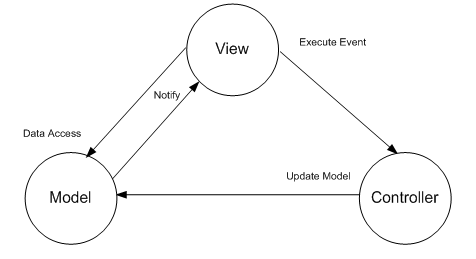
\includegraphics[scale=0.4]{sections/arquitectura/mvc.png}
%\centering
%\caption{Model-Vista-Controlador}
%\label{fig:arquitectura_mvc}
%\end{figure}
%\newline L'arquitectura en aquest cas, ve donada pel mateix \textit{framework} que s'ha fet servir per al desenvolupament  (AngularJS).\\
%Per fer-ne un breu resum, seguint l'arquitectura anteriorment exposada, el \textit{frontend} s'estructura en tres grups.\\
%\newline Per una banda el \textbf{model}, donat que el client web no disposa d'\textit{storage} pròpi, entendrem com a model el component dins del projecte que s'encarrega de realitzar les peticions al \textbf{backend} i rebre'n els resultats (ja siguin satisfactoris o no).\\
%\newline Per l'altre banda la \textbf{vista}, que es tracta de la part visual, aquella que rep les interaccions de l'usuari i les transmet cap a la següent, i última capa, el controlador.\\
%\newline El \textbf{controlador} s'encarrega d'interpretar les interaccions realitzades per l'usuari i actuar en conseqüència. Aquestes actuacions poden oscil·lar entre amagar o deshabilitar elements de la pantalla, demanar dades al model per pintar-les per pantalla, entre altres.
%\subsubsection{Diagrama de casos d'ús}
%\begin{figure}[h]
%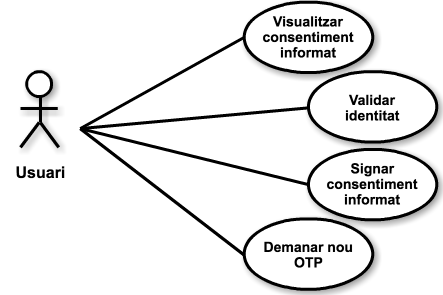
\includegraphics[scale=0.4]{sections/arquitectura/frontend_usecase.png}
%\centering
%\caption{Casos d'ús \textit{frontend}}
%\label{fig:cas_us_frontend}
%\end{figure}
%La Figura \ref{fig:cas_us_frontend} mostra els diferents casos d'ús del mòdul desenvolupat que pot dur a terme un usuari client.\\
%\newline L'objectiu principal del \textit{frontend}, és permetre rebre a l'usuari les dades necessàries tals com el consentiment informat i el \textit{feedback} necessari per saber si l'operació de signatura s'ha dut a teme amb èxit o no. En cas de negatiu, s'ha de mostrar el missatge d'error pertinent.\\
%\newline Així doncs, la part client del projecte té els següents propòsits:
%\begin{enumerate}
%    \item Permetre la visualització i descàrrega del consentiment informat.
%    \item Permetre a l'usuari la signatura del consentiment, si així ho desitja.
%    \item Permetre a l'usuari demanar un nou codi OTP, en cas de que el que hagi rebut prèviament via SMS hagi caducat.
%\end{enumerate}
%Totes les operacions anteriors, es tradueixen a tot un seguit de crides HTTP a un backend mitjançant els mètodes GET i POST.
%\subsection{Backend}
%Està pensat i desenvolupat com una API Rest que dóna accés als recursos emmagatzemats a la base de dades, a través d'unes rutes (o \textit{endpoints}) definides als controladors.\\
%\newline L'acés a les rutes es realitza a través d'HTTP, fent ús dels mètodes \textit{GET}, \textit{POST}, \textit{PUT} i \textit{DELETE}, anàlogament, podriem dir que corresponen als mètodes \textit{CRUD}\footnote{\textbf{C}reate \textbf{R}ead, \textbf{U}pdate i \textbf{D}elete} d'una base de dades.\\
%\newline A nivell d'arquitectura, no es pot dir que faci ús d'una arquitectura pròpiament dita, per contra, fa ús de tot un seguit de conceptes d'enginyeria del software que tenen com a objectiu la producció d'un còdi net, mantenible i sobre tot, ben estructurat.
%Concretament, els conceptes són: \textit{clean architecture}, \textit{SOLID} i \textit{TDD}.\\
%\clearpage
%\subsubsection{Clean Architecture}
%\begin{figure}[h]
%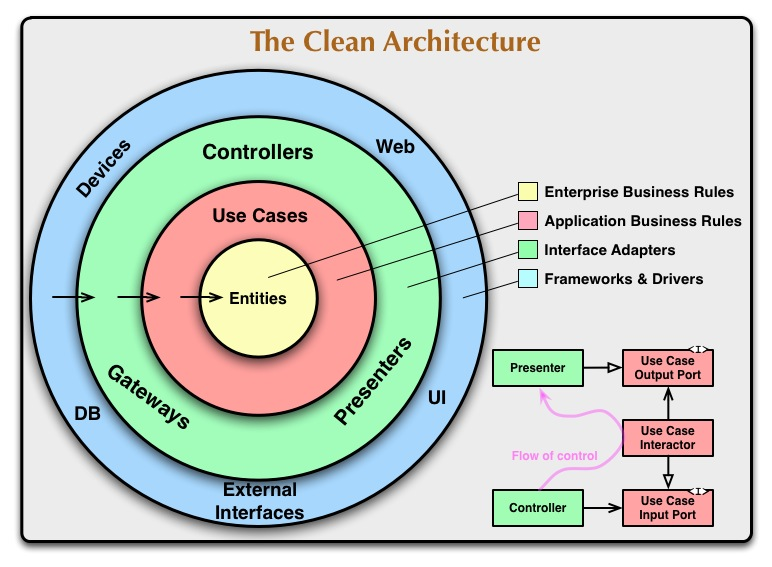
\includegraphics[scale=0.4]{sections/arquitectura/cleanArchitecture.jpg}
%\centering
%\caption{Clean Architecture}
%\label{fig:clean_architecture}
%\end{figure}
%La figura anterior (Figura \ref{fig:clean_architecture}), ens presenta un model conceptual on les diferents capes són independents les unes de les altres. La capa més interna, no coneix a la capa més externa i viceversa, obligant l'aplicació de patrons \textit{adapter} per la comunicació entre capes. \\
%\newline D'aquesta forma s'aconsegueix un codi amb una granularitat elevada, fàcil de mantenir donat el poc solapament que hi ha entre els diferents components del projecte, i amb components fàcilment substituïbles.\\
%\subsubsection{S.O.L.I.D}
%És l'acrònim de:
%\begin{itemize}
%    \item \textit{\textbf{S}ingle responsability}
%    \item \textit{\textbf{O}pen close}
%    \item \textit{\textbf{L}iskov substitution}
%    \item \textit{\textbf{I}nterface segregation}
%    \item \textit{\textbf{D}ependency inversion}
%\end{itemize}
%Els cinc punts anteriors, són un seguit de convencions, un seguit d'idees enfocades a la producció d'un codi net, estructurat i fàcil de mantenir.\\
%\newline Per aconseguir-ho, treballa amb idees tals com la responsabilitat única de les classes, classes obertes a l'extensió, però no a la modificació, injecció de dependències, ús de interfícies a mode de contracte, etc.\\
%\newline Són tot un seguit de regles que funcionen perfectament amb les idees presentades anteriorment referents a la \textit{Clean Architecture}

%\newline L'arquitectura representada, és l'arquitectura clàssica d'un servei web en el més estricte sentit de la paraula.\\
%\newline La figura anterior (Figura \ref{fig:arquitectura_global}) respon al que coneixem com arquitectura web.\\
%\newline Parlant en termes generals, l'arquitectura mostrada anteriorment es basa en un client que fa peticions a una infraestructura, normalment i donats els temps que corren en forma de API Rest, que fa d'intermediari entre aquest client i la part del model de dades, generalment la base de dades del projecte, i tot englobat dins del mateix paquet.\\
%\newline Situant-nos en un context més actual amb les diferents llibreries existents i amb diversitat d'arquitectures, cada una enfocada a donar solució a un problema concret, podríem dir que realment ens trobem amb una arquitectura similar a la mostrada a la Figura \ref{fig:arquitectura_global}.
%\newline L'exemple anterior, ens mostra dos components separats. Ambdós amb la seva pròpia arquitectura i comunicats generalment entre ells motjançant HTTP \footnote{Hypertext Transfer Protocol} i els mètodes \textit{GET}, \textit{POST}, \textit{PUT} i \textit{DELETE}.\\
%\newline La gran majoria de projectes actuals, es composen principalment de dos elements: un \textit{frontend} (client), en el nostre cas executat sobre un navegador web a través de la qual l'usuari final interactua amb tot el sistema, i un segon element, anomenat \textit{backend}, normalment en format API, la funció del qual és, a través d'un seguit de mètodes, permetre al client servir-se de les dades emmagatzemades en el moment que ho necessiti.\\
%\newline En el nostre cas particular, el \textit{frontend} del projecte respon a una arquitectura MVC \footnote{Model View Contoller} com es mostra a la figura \ref{fig:arquitectura_mvc}